\par O conceito de densidade de estados ($\rho(E)$) consiste no número de estados por volume no espaço $k$. A densidade de estados aparece em diversas áreas da Física, como, por exemplo, na termodinâmica e na óptica, na dedução da Lei de Planck para calcular densidade de estados de fótons. Em física estatística, para calcular densidades de energia nos sistemas físicos, e na mecânica quântica para calcular as probabilidades de transição envolvendo estados em um contínuo de energia, por exemplo\cite{confinamento2}.

\par Essa densidade de estados é dada por:

\begin{equation}
	\label{confinamento_2}
	\rho(E) = \frac{dN}{dE},
\end{equation}
em que $N$ é o número total de estados por espaço e $E$ é a energia do estado.

\par A densidade de estado pode ser analisada para os casos de três, duas, uma e zero dimensões livres, como podemos ver na tabela presente na figura \ref{fig10}:

\begin{figure}[H]
  \caption{Classificação de estruturas confinadas}
  \centering
  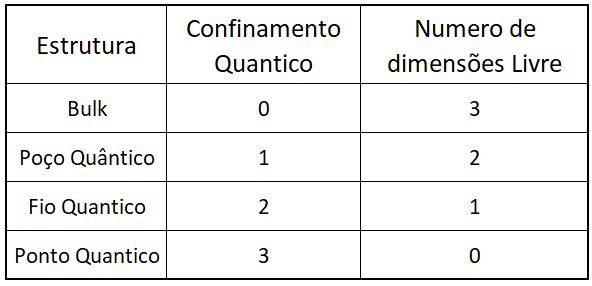
\includegraphics[width=0.65\textwidth]{images/figura10.jpg}
  \label{fig10}
\end{figure}

\par Nesse tópico do trabalho será analisada a densidade de estados para os pontos quânticos, que consiste no caso de zero dimensões livres (0D). Porém, para que fique mais claro o argumento utilizado para obtenção da expressão matemática que rege a densidade de estados no caso 0D, é conveniente que se entenda como se obtém a densidade de estado para qualquer dimensão livre. Por exemplo, utilizaremos o caso mais simples, que consiste em apenas uma dimensão livre (1D), nos chamados fios quânticos.

\begin{figure}[H]
  \caption{Fio quântigo inserido no espaço recíproco $k$}
  \centering
  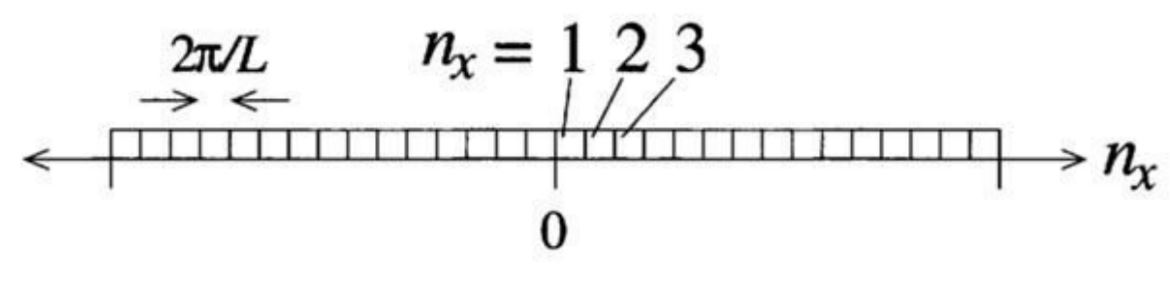
\includegraphics[width=0.8\textwidth]{images/figura11.jpg}
  \label{fig11}
\end{figure}

\par O número de estados $N$ é igual ao comprimento do fio ($2k$), dividido pelo comprimento ocupado por um estado $\left(\frac{2\pi}{L}\right)$ e dividido pelo comprimento no espaço real. Tem-se\cite{confinamento3} então

\begin{equation}
	\label{confinamento_3}
	N = 2k \cdot \frac{1}{\frac{2\pi}{L}} \cdot \frac{1}{L} \cdot 2
\end{equation}
onde o fator 2 surge devido à degeneração do spin.

\par Logo, N e sua derivada:

\begin{align}
	\label{confinamento_4}
	N^{1D} = \frac{4k}{2\pi}\\
	\frac{dN^{1D}}{dk} = \frac{2}{\pi}		
\end{align}

\par Portanto, definindo a densidade de estados utilizando a regra da cadeia
\begin{equation}
	\label{confinamento_5}
	\rho^{1D}(E) = \frac{dN^{1D}}{dE} = \frac{dN^{1D}}{dk}\ \frac{dk}{dE}
\end{equation}

%TODO - REFERENCIAR
\par É possível calcular o termo $\frac{dk}{dE}$ utilizando a energia do elétron livre dada na equação REFERENCIAR

\begin{equation}
	\label{confinamento_6}
	 \frac{dk}{dE} = \left(\frac{2m^{\ast}}{\hbar^2}\right)^{\frac{1}{2}} \frac{E^{-\frac{1}{2}}}{2}
\end{equation}

\par Da equação \eqref{confinamento_4} e \eqref{confinamento_6}, subsititui-se em \eqref{confinamento_5}
\begin{align}
	\label{confinamento_7}
	\rho^{1D}(E) &= \frac{2}{\pi} \left(\frac{2m^{\ast}}{\hbar^2}\right)^{\frac{1}{2}} \frac{E^{-\frac{1}{2}}}{2}\\
	\rho^{1D}(E) &= \left(\frac{2m^{\ast}}{\hbar^2}\right)^{\frac{1}{2}} \frac{1}{\pi E^{-\frac{1}{2}}},
\end{align}
sendo esta, a densidade de estado para 1D.

\par De forma análoga, obtém-se os valores das desnidades de estado para todas as dimensões. A tabela expressa na figura mostra os resultados:

\begin{figure}[H]
  \caption{Tabela das densidades de estado para as três dimensões. Extraído de \cite{confinamento3}}
  \centering
  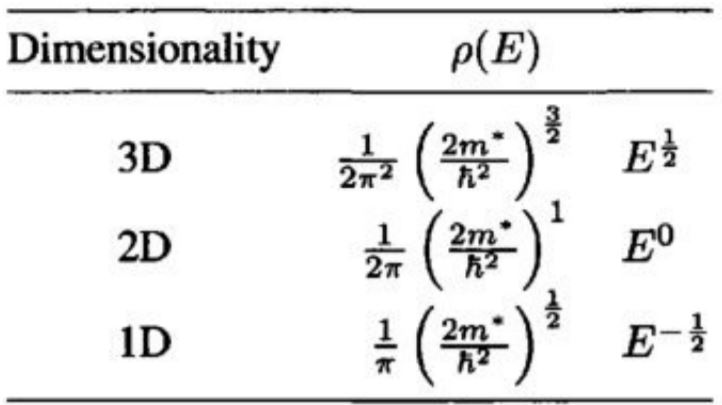
\includegraphics[width=0.6\textwidth]{images/figura12.jpg}
  \label{fig12}
\end{figure}

\par No entanto a situação para os pontos quânticos é diferente. Como o elétron no ponto quântico está confinado nas 3 dimensões, não há espaço $k$ para ser preenchido e todos os estados disponíveis existem apenas em energias discretas. Portanto, pode-se descrever a densidade de estados com o \textbf{delta de Dirac}. 

\begin{equation}
	\label{confinamento_8}
	 \rho(E)_{0D} = 2\delta(E-E_{c}),
\end{equation}
onde $\delta$ representa o delta de Dirac e $E_{c}$ é a energia de confinamento do elétron.

\par A figura  apresenta gráficos indicadores de densidade de estado para todas as dimensões.

\begin{figure}[H]
  \caption{Gráficos da densidade de estado em todas as dimensões}
  \centering
  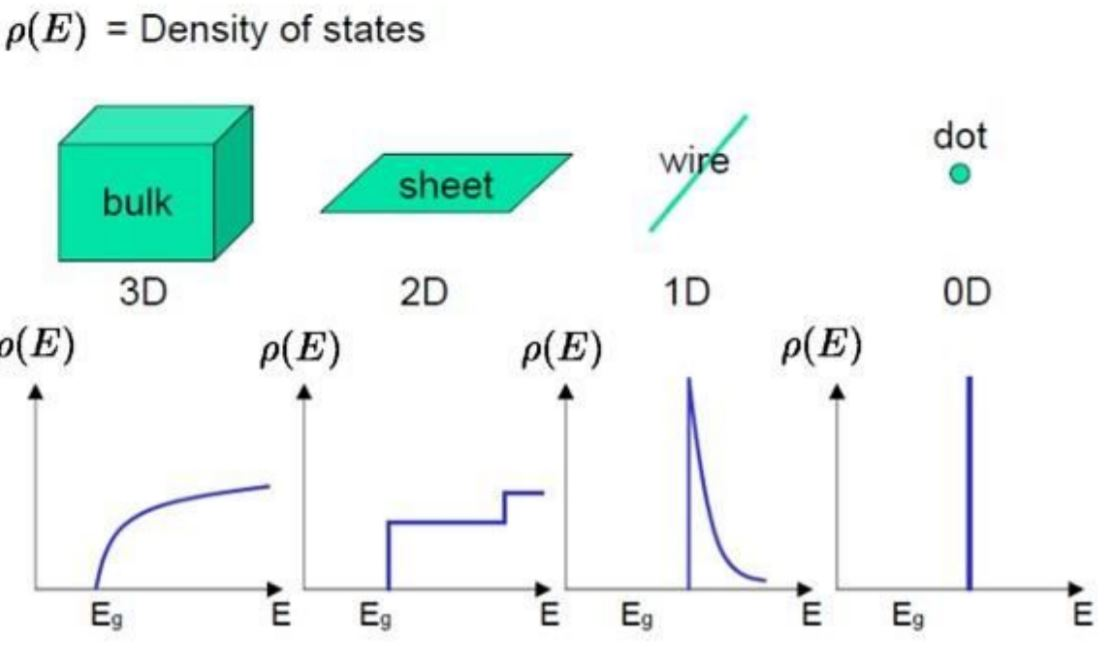
\includegraphics[width=0.6\textwidth]{images/figura13.jpg}
  \label{fig13}
\end{figure}

\par Observando os resultados de densidade de estados para os pontos quânticos, comprova-se que de fato existem apenas alguns níveis de energia bem definidos e discretos nos quais o elétron pode ocupar um estado. O ponto quântico pode, por isso, ser chamado de átomo artificial. 